\documentclass{article}
\usepackage[utf8]{inputenc}
\usepackage{mathrsfs}
\usepackage{abstract} 
\usepackage[spanish,es-noshorthands]{babel}
\usepackage[margin=2cm]{geometry}
\usepackage{enumitem}
\usepackage{amsmath,amsthm,amssymb} 
\usepackage{graphicx}
\usepackage{pdfpages}
\usepackage{gensymb}
\usepackage{comment}
\usepackage{longtable}
\spanishdecimal{.}
\usepackage{titling}
\usepackage{float}
\usepackage{tikz}
\usetikzlibrary{arrows,scopes}
\usepackage{xcolor}
\usetikzlibrary{calc}
\usepackage{mathrsfs}
%\newcommand{\U}[1]{\, \mathrm{#1}} %comando que formatea las unidades con el espaciamiento correcto y en romanas
\usepackage{calligra}
\DeclareMathAlphabet{\mathcalligra}{T1}{calligra}{m}{n}
\DeclareFontShape{T1}{calligra}{m}{n}{<->s*[2.2]callig15}{}
\usetikzlibrary{positioning}
\usetikzlibrary{shapes.geometric}
\usetikzlibrary{shapes.misc}
\usepackage{xcolor}
\usepackage{textcomp}
\usepackage{gensymb}
\usepackage{url}
\setlength{\parskip}{10px}
\usepackage{fancyhdr}
\pagestyle{fancy}
\setlength{\headheight}{20pt}



\title{\textbf{Análisis de Datos de Diabetes}}

\author{
  García, Juan Manuel\\
  \texttt{first1.last1@xxxxx.com}
  \and
  Herrera, José Emiliano\\
  \texttt{eherrera1331@gmail.com}
  \and
  Miramontes, Fred\\
  \texttt{liloliol@hotmail.com}
  \and
  Román, Christopher\\
  \texttt{ferrobin34@gmail.com}
  \and
  Sánchez, Gabriel\\
  \texttt{178294@iberopuebla.mx}
  \and
  Sánchez, Ludim\\
  \texttt{sanchezludim.anel@gmail.com}
}



\date{\today}


\begin{document}
%\maketitle
\twocolumn

\twocolumn[
  \begin{@twocolumnfalse}
    \maketitle
    \vspace*{-1cm}
    \begin{center}\rule{0.9\textwidth}{0.1mm} \end{center}
    \begin{abstract}
    En esta práctica se identificaron los productos, partículas resultantes, de una colisión de un haz de protones con un gas de $SF_6$, mejor conocido como \emph{hexafloruro de azufre}. Dichos productos fueron los siguientes iones: $F^+$, $SF^+$, $S^+$, $SF_2^{++}$, $SF^+$, $SF^+_2$, $SF^+_3$, $SF^+_4$ y $SF^+_5$, resultando éste último el más abundate. Los iones anteriores fueron identificados a través de su \emph{Relación Masa/Carga}, sin embargo no se notó presencia de iones $SF_6$, esto puede deberse a su configuración electrónica poco estable. Las colisiones se llevaron a cabo en el \emph{acelerador lineal} de bajas energías ($1\ keV$ a $10\ keV$) que se encuentra en el edificio \emph{Tlahuizcalpan} de la Facultad de Ciencias de la Universidad Nacional Autónoma de México. Además, en ésta práctica se discute el funcionamiento de las partes del acelerador lineal, así como la razón de la ausencia del ión $SF_6$.
    \end{abstract}
    \begin{center}\rule{0.9\textwidth}{0.1mm} \end{center}
    \vspace*{1cm}
  \end{@twocolumnfalse}
]

\section{Introducción}
La diabetes es una enfermedad crónica en la que el cuerpo no es capaz de regular la cantidad de glucosa en la sangre. La glucosa en la sangre es la principal fuente de energía y ésta proviene de los alimentos. Con el transcurso del tiempo, el exceso de glucosa en la sangre puede causar problemas de salud, tales como enfermedades del corazón, daño a los nervios y enfermedad de los riñones.

Los principales factores de riesgo de la diabetes son:
\begin{itemize}
	\item \textbf{Peso:} Mientras más tejido graso, más resistentes serán las células a la insulina.
	\item \textbf{Inactividad:} Mientras menos actividad se realice, mayor será el riesgo. La actividad física ayuda a controlar el peso, utiliza la glucosa como energía y hace que tus células sean más sensibles a la insulina.
	\item \textbf{Antecedentes familiares:} El riesgo se incrementa si padres o hermanos tienen diabetes tipo 2.
	\item \textbf{Raza o grupo étnico:} Aunque no está claro por qué, personas de ciertos orígenes, como las personas negras, hispanas, los indígenas estadounidenses y asiático-americanas, corren un mayor riesgo.
	\item \textbf{Edad:} El riesgo aumenta con la edad. Esto puede deberse a que la actividad física es menor, se pierde masa muscular y se aumenta de peso a medida que envejeces. Sin embargo la diabetes tipo 2 también está aumentando entre los niños, los adolescentes y los adultos jóvenes.
	\item \textbf{Presión arterial alta:} Una presión arterial de más de $140/90$ milímetros de mercurio (mm Hg) implica un alto riesgo de desarrollar diabetes tipo 2.
	\item \textbf{Niveles anormales de colesterol:} Si se cuenta con niveles bajos de lipoproteínas de alta densidad o de colesterol ``bueno", el riesgo de desarrollar diabetes tipo 2 será mayor. Lo triglicéridos son otro tipo de grasas que se transportan en la sangre. Las personas con niveles altos de triglicéridos afrontan un riesgo elevado de padecer diabetes tipo 2. 
\end{itemize}

Desde el año 2000, la diabetes mellitus en México es la primera causa de muerte entre las mujeres y la segunda entre los hombres. En 2010, esta enfermedad causó cerca de 83,000 muertes en el país. Es por esto que decidimos hacer un análisis sobre este problema.


\section{Objetivos}

Teniendo en cuenta el contexto y la importancia del estudio de esta enfermedad se plantean las siguientes preguntas:
\begin{itemize}
	\item ¿Existe alguna relación entre la diabetes y el grosor de la piel?
	\item ¿Existe alguna relación de la diabetes con la edad?
	\item Observar la correlación entre los factores anteriormente mencionados y la diabetes.
	\item ¿Existe alguna relación entre el embarazo y la diabetes?
	\item ¿Quienes son más propensos a contraer esta enfermedad, hombres o mujeres?
	\item ¿Qué factor de riesgo hay que tener más en cuenta para evitar contraer diabetes?
\end{itemize}


\section{Dataset}

El dataset utilizado contiene datos recopilados del \emph{National Institute of Diabetes and Digestive and Kidney Diseases} y se puede consultar en la siguiente liga \url{https://www.kaggle.com/mathchi/diabetes-data-set}. Cada registro contiene ciertos parámetros de mujeres de la India de, al menos 21 años. Los campos del dataset son los siguientes:

\begin{itemize}
	\item \textbf{Pregnancies:} Número de veces que se ha embarazado.
	\item \textbf{Glucose:} Concentración de glucosa en plasma a dos horas en un test oral de tolerancia a la glucosa. 
	\item \textbf{BloodPressure:} Presión sanguínea.
	\item \textbf{SkinThicness:} Grosor de la piel del tricep.
	\item \textbf{Insulin:} Suero de insulina.
	\item \textbf{BMI:} Índice de masa corporal.
	\item \textbf{DiabetesPedigreeFunction:} Diabetes pedigree function.
	\item \textbf{Age:} Edad.
	\item \textbf{Outcome:} 0 o 1.
\end{itemize}


\section{Limpieza de los datos}

En general, el dataset se encontraba muy limpio, a excepción de unos valores NaN.

\begin{figure}[H]
	\centering
	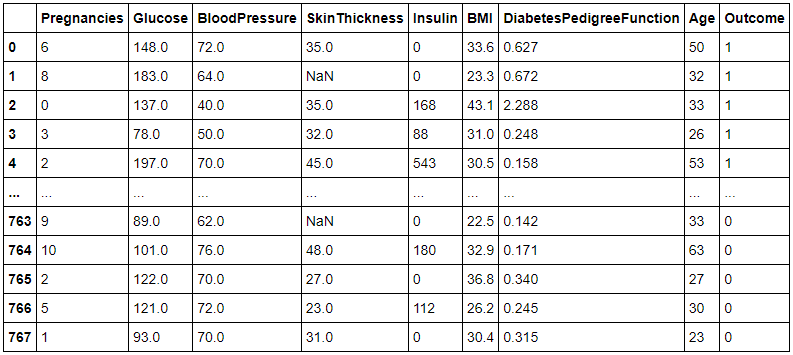
\includegraphics[width=0.9\linewidth]{dataset_sucio.png}
	\caption{Dataset con el que se va a trabajar.}%
	\label{fig:dataset_sucio}
\end{figure}

Estos valores NaN se sustituyeron por $0$, resultando:

\begin{figure}[H]
	\centering
	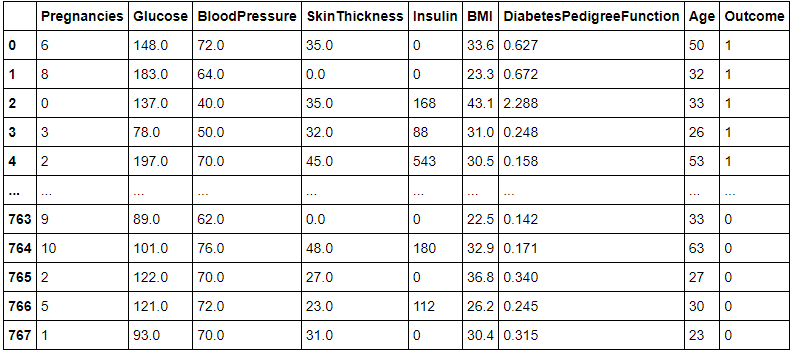
\includegraphics[width=0.9\linewidth]{dataset_limpio.png}
	\caption{Dataset ya ``limpio''}%
	\label{fig:dataset_limpio}
\end{figure}

Por último, al dataset se le agregó un nuevo campo llamado ``ComposicionCorporal'', denotado como ``cc'' en la ecuación [\ref{cc}], con variables categóricas que indican el nivel del índice de masa corporal, es decir:

\begin{equation}\label{cc}
	cc=
	\begin{cases}
		\text{Bajo, si      } BMI \leq 18.85\\
		\text{Normal, si    } 18.5 < BMI \leq 24.9\\
		\text{Elevado, si   } 24.9 < BMI \leq 29.9\\
		\text{Obesidad, si  } 29.9 < BMI
	\end{cases}
\end{equation}

Resultando:

\begin{figure}[H]
	\centering
	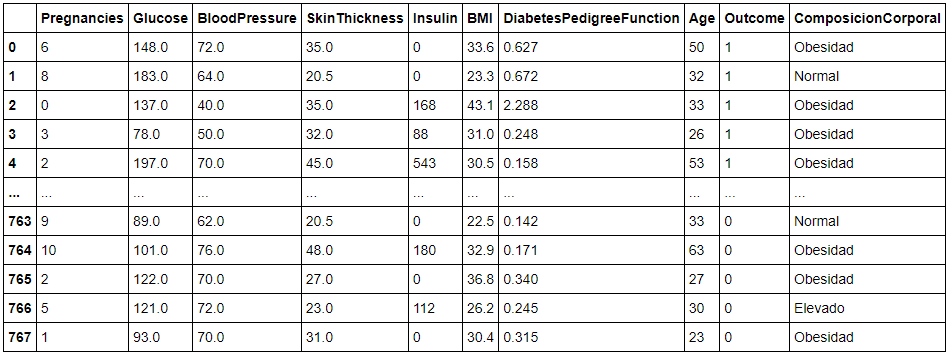
\includegraphics[width=0.9\linewidth]{dataset_completo.png}
	\caption{Dataset completo.}%
	\label{fig:dataset_completo}
\end{figure}


\section{Análisis Exploratorio}

Una vez se obtuvo el dataset [\ref{fig:dataset_completo}] procedemos a realizar un análisis exploratorio de los datos.

Lo primero que se observa es que, del total de la muestra, hay 500 mujeres ``sanas''\footnote{Entiéndase por sanas a mujeres que salieron negativas al examen de detección de la diabetes.} y 268 mujeres con diabetes detectada.

\begin{figure}[H]
	\centering
	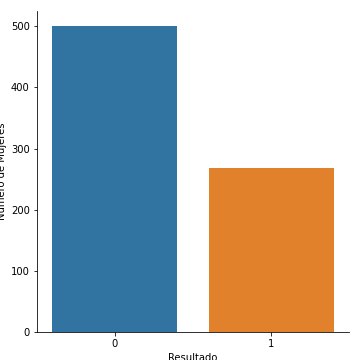
\includegraphics[width=0.65\linewidth]{bar_diabetes.png}
	\caption{Gráfica de barras que muestra la incidencia de diabetes en la muestra de población tomada.}%
	\label{fig:bar_diabetes}
\end{figure}

Cómo se muestra en la figura [\ref{fig:bar_diabetes}], el número 0 representa a una mujer \emph{sana} y 1 a una mujer con diabetes.

Por otro lado, y hablando en términos generales de la muestra, se observa que la mayoría de los registros corresponden a mujeres jóvenes entre 21 y 36 años, figura [\ref{fig:edad_muestra}]. 

\begin{figure}[H]
	\centering
	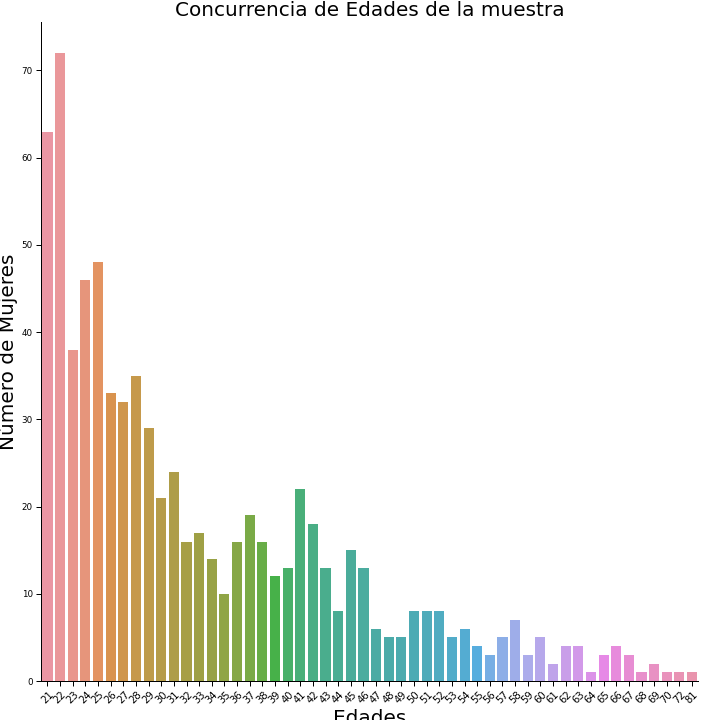
\includegraphics[width=0.65\linewidth]{edad_muestra.png}
	\caption{Edad de mujeres de la muestra.}%
	\label{fig:edad_muestra}
\end{figure}

Graficando de nuevo la concurrencia de edades pero ahora separadas según su diagnóstico

\begin{figure}[H]
	\centering
	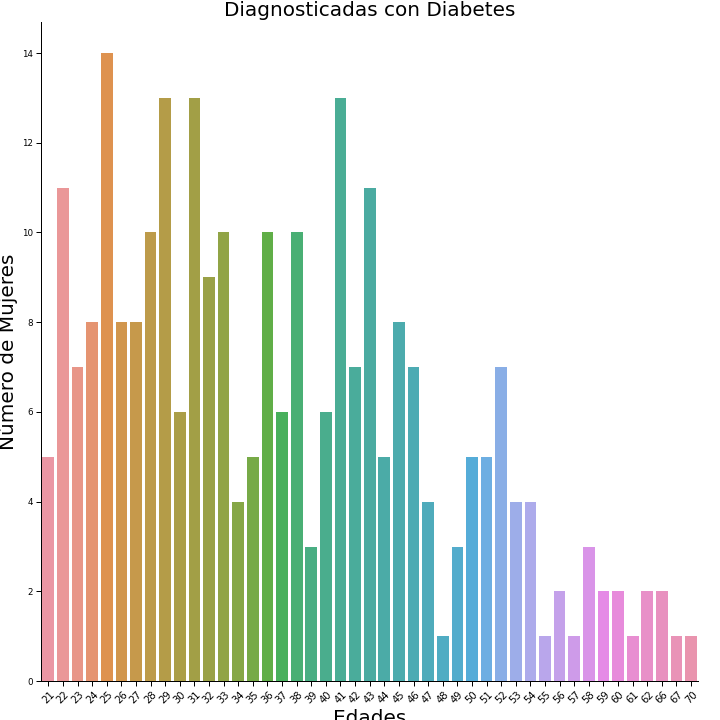
\includegraphics[width=0.65\linewidth]{edad_diabetes.png}
	\caption{Gráfica de la concurrencia de edades de mujeres con diabetes.}%
	\label{fig:edad_diabetes}
\end{figure}

\begin{figure}[H]
	\centering
	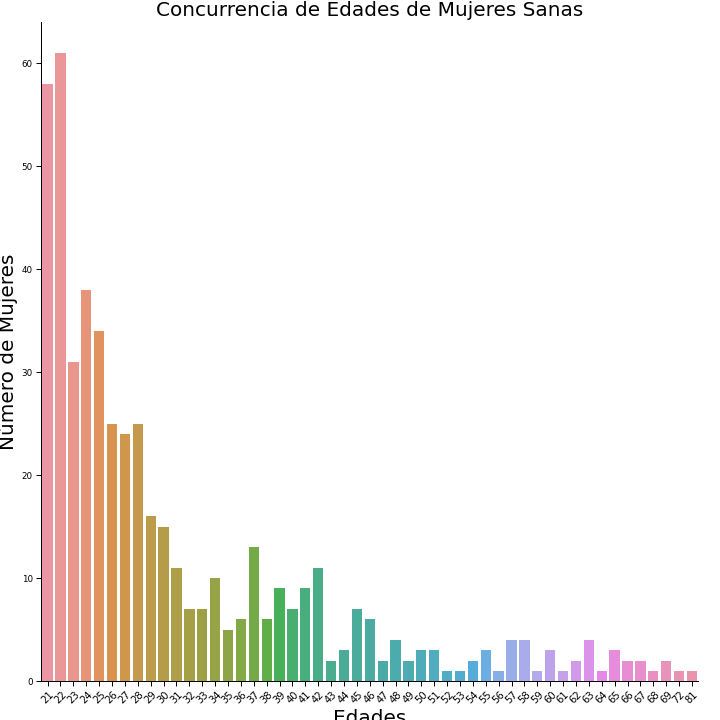
\includegraphics[width=0.65\linewidth]{edad_no_diabetes.png}
	\caption{Gráfica de la concurrencia de edades de mujeres sanas.}%
	\label{fig:edad_no_diabetes}
\end{figure}

Como se observa en la figura [\ref{fig:edad_diabetes}] la distribución de mujeres con diabetes según su edad parece tener una distribución distinta a la mostrada en la figura [\ref{fig:edad_no_diabetes}]. Para la primera gráfica [\ref{fig:edad_diabetes}], parece que los casos se distribuyen normalmente\cite{Distro_normal} y para la gráfica [\ref{fig:edad_no_diabetes}] se tiene lo que parece ser un decaimiento exponencial. Esto se debe a que, como ya se mencionó, la mayoría de las mujeres registradas son jóvenes.




\onecolumn{
  \bibliographystyle{abbrv}
  \bibliography{bibliografia}
}

\end{document}

